\subsection{Bracketing Methods - Chapter 5}

\begin{enumerate}

\item {\bf Graphical Approach}

It is possible to obtain the root of a function by simply plotting it
and zooming in on the graph. If we return to our example where we
simulate the ball flying through the air and zoom in on the graph we
see that the ball collides with the ground around 10 meters. This
results in a time of 1.4142.

\begin{figure}[htb]
  \begin{center}
    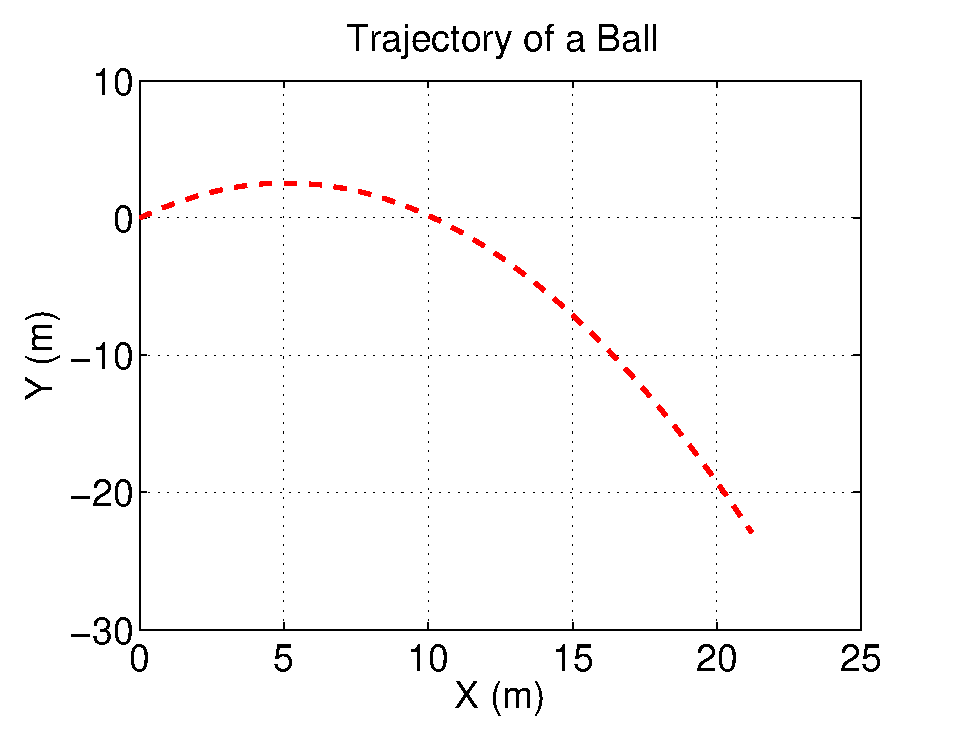
\includegraphics[height=0.45\textwidth,width=0.6\textwidth]{Graphics/Example_Plot}
  \end{center}
\end{figure}

Numerical computation of the point where the ball hits the ground is
equal to 10.194 meters which corresponds to a time of 1.4416. Thus
graphically we were not off by very much. However, this does not help
us very much when it comes to finding a better solution.

\item{\bf Bisection Method}

The best way to describe the bi-section method is the shower heat
problem. When you jump in your always turn the knob all the way up to
heat the water up. But you jump in and it's way too hot. So you turn
it down. More than likely it's too cold now. So you turn it back but
not as much as before. You repeat this turning back and forth until
you dial in the right temperature. This is much like the bi-section method.

When you looked at the graph and searched for the root you inherently
looked for where the line changed sign. That is when the value of y
went from positive to negative you picked off the point. It is
possible to do this while using a stepping algorithm. That is we can
start at an initial guess of t = 1. $y(t=1) = v_yt - (1/2)gt^2 =
2.166 > 0$. Since y is greater than 0 we can try a new guess such that
$t_1 = t_0 + \Delta t$. If we choose $\Delta t = 0.5$ our new guess is
then $t_1 = 1.5$. Our height is then $y(t=1.5) = -0.42965 < 0$. Thus
our time that we hit the ground must be inbetween 1 and 1.5
seconds. At this point we can divide our timestep by 2 and compute a
new timestep of 0.25. Our new time is then $t=1.25$ and $y(t=1.25) =
1.1748$ which is greater than zero thus our estimate lies inbetween
1.25 and 1.5. We again half our step such that we compute our time at
$t=1.375$ and $y=0.4492$. Our value of y is still greater than zero
thus we step forward one more time and get $t=1.5$. We know that this
value has a height that is less than zero which means our function has
switched signs and we then halve our timestep again to $1/16$ and
compute $t=1.5-1/16=1.4375$. This process repeats itself over and over
again until a convergence criterion is met. A computer code can be
used to run the bisection method. The algorithm is given below.

\begin{framed}
\textcolor{blue}{function} ti = bisection()

clc

close all

\textcolor{OliveGreen}{\%Initial guess}

ti = 1;

\textcolor{OliveGreen}{\%Initial timestep}

dt = 0.5;

\textcolor{OliveGreen}{\%Initial Function Value}

f1 = myfunc(ti);

f2 = f1;

\textcolor{OliveGreen}{\%Set an error threshold}

threshold = 1e-2;

\textcolor{OliveGreen}{\%Loop while error is greater $>$ threshold}

\textcolor{blue}{while} abs(f1-0) $>$ threshold

~~~~~~~\textcolor{OliveGreen}{\%Step forward until function changes sign}

~~~~~~~\textcolor{blue}{while} sign(f2) == sign(f1)

~~~~~~~~~~~~~~ti = ti+dt; 

~~~~~~~~~~~~~~f2 = myfunc(ti);

~~~~~~~\textcolor{blue}{end}

~~~~~~~\textcolor{OliveGreen}{\%If the loop breaks out we change the sign of dt and halve it}

~~~~~~~dt = -0.5*dt;

~~~~~~~\textcolor{OliveGreen}{\%Furthermore we change f1 to f2}

~~~~~~~f1 = f2;

\textcolor{blue}{end}

\textcolor{blue}{function} y = myfunc(t)

V = 10;

theta = pi/4;

vy = V*sin(theta);

a = -9.81;

y = vy*t + (1/2)*a*t\textrm{\^}2;

\end{framed}

Running the code below produces the following table of data. Notice
that to get our error to 1e-2 only requires 10 iterations.

\begin{center}
\begin{tabular}{l | l l l l l l l l l l}
Iteration & 1 & 2 & 3 & 4 & 5 & 6 & 7 & 8 & 9 & 10  \\
\hline
t (sec) & 1.5 & 1.25 & 1.375 & 1.5 & 1.4375 & 1.469 & 1.4531 & 1.4375
& 1.445 & 1.441 \\
\hline
dt (sec) & 0.5 & -0.25 & 0.125 & 0.125 & -0.0625 & 0.031 & -0.016 &
-0.016 & 0.008 & -0.004 \\
\hline
y (m)  & -0.429 & 1.175 & 0.449 & -0.429 & 0.029 & -0.196
& -0.082 & 0.029 & -0.026 & 0.0014 \\
\end{tabular}
\end{center}

\item {\bf Bisection Method Alternate Approach}

It is possible to simple use an iterative method to solve for the
bisection method which students find to be much simpler. The algorithm is shown below:

\begin{enumerate}

\item Define upper(xU) and lower(xL) bounds 

\item Set initial conditions

\begin{equation}\nonumber
\begin{matrix}
\Delta x_1 = (xU-xL)/2 && x_1 = xL && y_1 = f(x_1) 
\end{matrix}
\end{equation}

\item Perform iterations using the following two iterative equations
  
\begin{equation}\nonumber
\begin{matrix}
x_{n+1} = x_n + \Delta x_n && \Delta x_{n+1} = \Delta x_n /2
\end{matrix}
\end{equation}

\item Change the sign of $\Delta x_{n+1}$, if $sign(f(x_n)) \sim= sign(f(x_{n+1}))$

\end{enumerate}

\begin{framed}

If you're looking for a fun game to test out your bi-section skills
check out the clock game from the Price is Right. Here are two really fun
links. 

{\bf Terrible Bi-Section Contestant:} \url{https://www.youtube.com/watch?v=oc9H8bo8yg0}\\
{\bf Million Dollar Winner:}
\url{https://www.youtube.com/watch?v=RJw1rlmJ81U}

\end{framed}

\item{\bf The Parachutist}

  An interesting example that uses the Bi-Section method is the falling
  parachutist with unknown drag coefficient. If we use the simplest
  form of Newton's Second Law we have

  \beq
  \sum{F} = ma
  \eeq

  where F is the forces on the parachutist. In this example the only
  forces are gravity and aerodynamic forces. To simplify this problem
  we assume Newtonian drag such that $F_d=-cv$ where $c$ is a drag
  coefficient and $v$ is the velocity of the parachutist. We can also
  use the relationship that $\dot{v}=a$ so that our equation of motion
  is given as

  \beq
  \dot{v}+(c/m)v=g
  \eeq

  This equation can be solved analytically using methods from
  Differential equations. I recommend you brush up on your
  differential equation skills before you move on. The analytical
  solution is given below to check your work where $v_0$ is the
  initial velocity of the parachutist.

  \beq
  v(t) = v_0e^{-ct/m}+(1-e^{-ct/m})mg/c
  \eeq

  So where does the bi-section method come in? Let's say that a
  velocity sensor is put on the parachutist so that $v_0$ is known,
  and $v(t=4)$ is also known. 

  \beq
  v_0e^{-4c/m}+(1-e^{-4c/m})mg/c - v(t=4) = 0
  \eeq
  
  In the equation above the only unknown is then the drag coefficient
  since gravity, and the mass of the parachutist are known. Since the
  equation above is in the form $v(c)=0$ the equation can be solved
  using the bi-section method. The solution is left as an example to
  the reader.

\item {\bf False Position Method}

The false position method starts with an initial guess that yields a
result that is less than zero and another value that is greater
than zero. A line is then connected between the two and where this
line intersects the zero line is the new value of the lower or upper
bound depending on the sign of the result. For example, the graph
below shows the first iteration of the example problem above.

\begin{figure}[htb]
  \begin{center}
    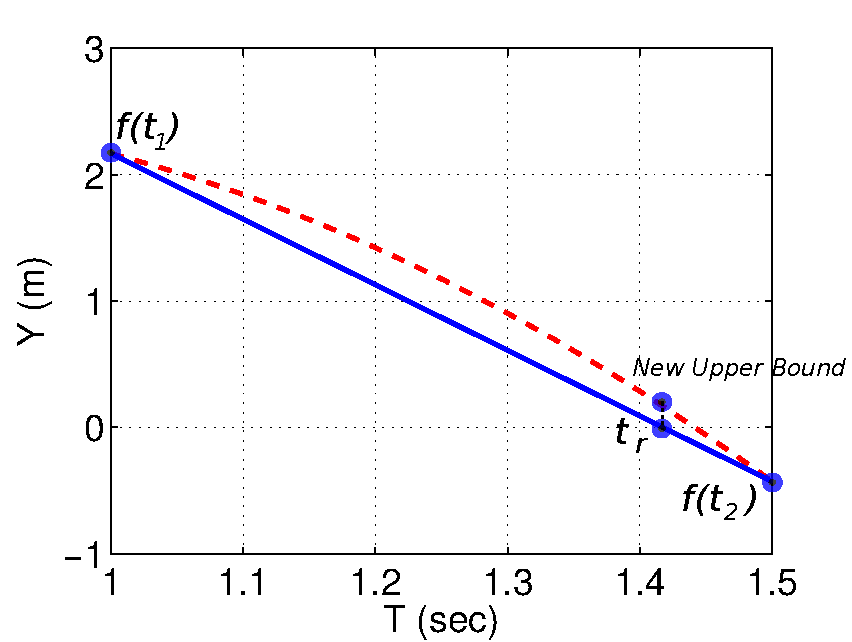
\includegraphics[height=0.45\textwidth,width=0.6\textwidth]{Graphics/False_Position.pdf}
  \end{center}
\end{figure}

Here $f(t_1)$ is positive and $f(t_2)$ is negative. A straight line
is then connected and $t_r$ is solved using the equation below which
is derived using the equation of a line.

\begin{equation} 
t_r = t_2 - \frac{f(t_2)(t_1-t_2)}{f(t_1)-f(t_2)}
\end{equation}

Using the new value of $t$ the sign of $f(t_r)$ is computed. Since it
is the same as $f(t_1)$, $t_r$ becomes the new upper bound and
$t_r=t_1$. A simple code can also be written to run the false position
method and is given below. Running this code only requires 8
iterations. It is apparent then that this method is faster for the
given problem. Doing a simply tic,toc test yields this result. Note
that a tic,toc test must be done numerous times such as a for loop to
test for convergence. 

\begin{framed}
\textcolor{blue}{function} falseposition()

clc

close all

\textcolor{OliveGreen}{\%Initial guess}

t1 = 1;

\textcolor{OliveGreen}{\%Initial timestep}

dt = 0.5;

t2 = t1 + dt;

\textcolor{OliveGreen}{\%Initial Function Value}

f1 = myfunc(t1);

f2 = myfunc(t2);

fr = f1;

\textcolor{OliveGreen}{\%Set an error threshold}

threshold = 1e-2;

\textcolor{OliveGreen}{\%Loop while error is greater than threshold}

\textcolor{blue}{while} abs(fr-0) $>$ threshold

~~~~~~~\textcolor{OliveGreen}{\%Compute tr based on f1 and f2}

~~~~~~~tr = t2 - f2*(t1-t2)/(f1-f2);

~~~~~~~fr = myfunc(tr);

~~~~~~~\textcolor{OliveGreen}{\%Test to see which bound we will replace}

~~~~~~~\textcolor{blue}{if} sign(fr) == sign(f1)

~~~~~~~~~~~~~~t1 = tr;

~~~~~~~\textcolor{blue}{else}

~~~~~~~~~~~~~~t2 = tr;

~~~~~~~\textcolor{blue}{end}

\textcolor{blue}{end}

\end{framed}

Another interesting test is to plot the error as a function of
iteration number. The figure below shows this. Notice how the
bisection method is all over the place whereas the false position
method is fairly linear.

\begin{figure}[htb]
  \begin{center}
    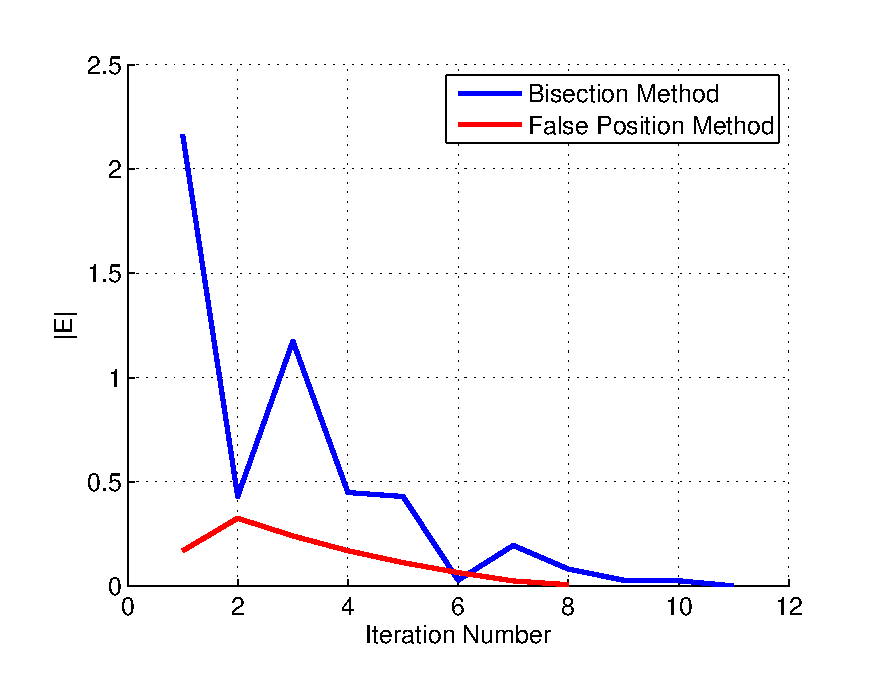
\includegraphics[height=0.45\textwidth,width=0.6\textwidth]{Graphics/Error_Comparison}
  \end{center}
\end{figure}

\end{enumerate}

